\documentclass[11pt]{article}

% Packages
\usepackage{amsmath}
\usepackage{float}
\usepackage{graphicx}
\usepackage{sidenotes}
\usepackage[a4paper,
innermargin=2cm,
textwidth=12cm,
marginparwidth=5cm,
marginparsep=1cm,
heightrounded,
]{geometry}

\let\oldemph\emph
\renewcommand{\emph}[1]{\oldemph{\textbf{#1}}\marginpar{\textbf{#1}}}


%% Draw line
\usepackage{tikzpagenodes}

\usepackage{atbegshi}

\def\drawcode{%
\tikz [remember picture, overlay] \draw
([xshift=.5cm]current page text area.north east)
--
([xshift=.5cm]current page text area.south east);}

\AtBeginDocument{% For the first page
\drawcode}

\AtBeginShipout{% For the remaining pages
\drawcode}

% Document
\begin{document}
    \section{Introduction}

    \emph{Gartner Hype Cycle}:
    \begin{itemize}
        \item \emph{Innovation trigger} future, commercial value unknown
        \item \emph{Peak of inflated expection} specific success stories with a lot of restrictions
        \item \emph{Through of Disillusionment} understanding of limitations of technology
        \item \emph{Slope of Enlightment} use understanding to develop commercially viable usage
        \item \emph{Plateau of Productivity} technology becomes mainstream
    \end{itemize}

    \begin{figure}[H]
        \centering
        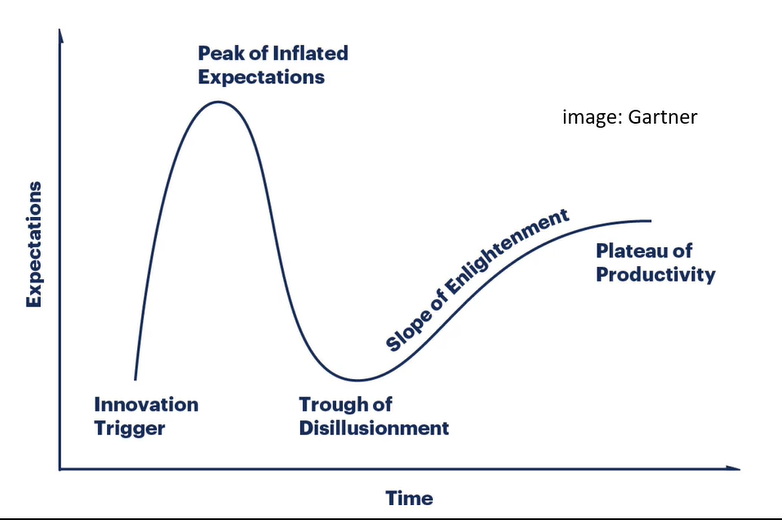
\includegraphics[width=0.5\textwidth]{img/hype.png}
        \caption{Hype}
        \label{fig:hype}
    \end{figure}

    \begin{figure}[H]
        \centering
        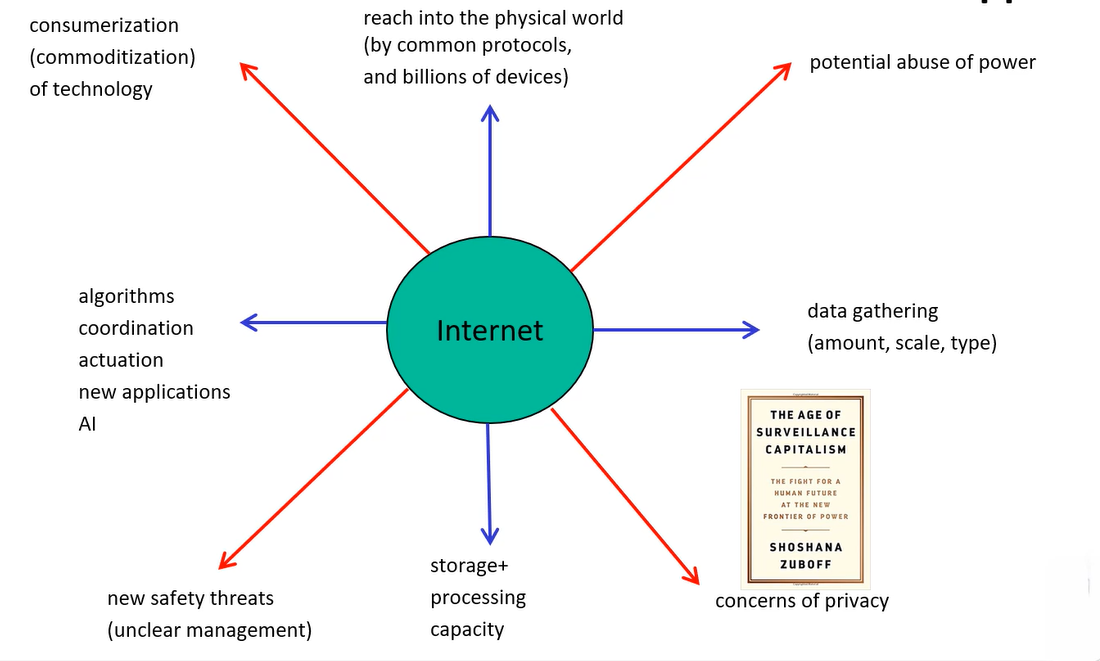
\includegraphics[width=0.5\textwidth]{img/internet.png}
        \caption{Internet}
        \label{fig:internet}
    \end{figure}

    Mainly focus on blue arrows in Fig~\ref{fig:internet}.

    \section{Examples}

    \subsection{Monitoring Energy Use example}

    \paragraph{Transformer}
    Report transformer data.
    \paragraph{Raspberry Pi}
    Create and provide overview report.
    Store data from smart meter.
    \paragraph{Smart meter}
    Report metering data.

    \paragraph{Questions}
    Which management concerns, which quality concerns, who owns the data,
    what interests are there in the data, who controls the data, what are the `things'?

    \paragraph{3 tier architecture}
    UI, application, database.
    Many websites work like this.




    
\end{document}